\chapter{Raccolta dati dei parcheggi}
\section{Procedura generale} 

\subsection{Raccolta}
Al fine di poter creare un classificatore per i tipi di parcheggio, la prima cosa
che è risultata necessaria è stata una raccolta di dati (una vista ad alto livello del
flusso di operazioni di raccolta è mostrata nella 
Figura~\ref{fig:flow_diagram_raccolta_dati}) di natura time-series.
In particolare, questi dati
dovevano essere di buona qualità, generati in maniera controllata e avere una chiara
classificazione che gli permetta di essere utilizzabili per un processo di training
\cite{pattern_extraction_time_series}.
Per questo motivo è stato importante che la raccolta fosse portata
avanti da poche persone fidate che fossero in grado di eseguire una serie di azioni
commettendo il minor numero di errori possibile.\\
\begin{figure}[]
    \centering
    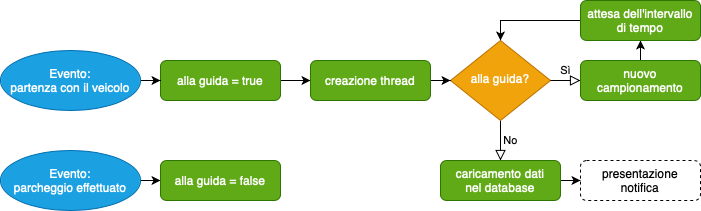
\includegraphics[width=14cm]{images/flow_diagram_raccolta_dati.png}
    \caption{Diagramma di flusso della raccolta dati.}
    \label{fig:flow_diagram_raccolta_dati}
\end{figure}
Dal momento che il modello classificatore in questione è destinato ad essere utilizzato
su applicativi mobile, e più in particolare sull'app GeneroCity, i dati che quest'ultimo
riceve come input devono provenire da sensori che si trovano direttamente sullo smartphone.
Così facendo, la modalità più ovvia di raccolta dei dati risulta essere 
quella di sfruttare gli stessi sensori dello smartphone
\cite{classification_smartphone_motion_sensors} \cite{driver_passenger_identification_smartphone}.\\
Coloro che hanno avuto il compito di raccogliere i dati, erano disposti di un sistema di
raccoglimento installato all'interno dell'app GeneroCity. Inizialmente, questo era presente
solo nella versione iOS\footnote{iOS page on Apple's website: 
\href{https://www.apple.com/ios}{\underline{link to the page.}}} dell'app, 
ma successivamente, è stato fatto il porting anche sulla
versione Android\footnote{Android's website: 
\href{https://www.android.com}{\underline{link to the page.}}}.
Questa operazione ha reso possibile che il numero di persone disponibili
per la raccolta di dati aumentasse significativamente.\\
Sfruttando alcuni eventi generati automaticamente dall'app, come ad esempio l'ingresso e
l'uscita dall'auto \cite{framework_user_experience_car}, è stato possibile avviare e 
interrompere la raccolta, senza troppa pressione o attenzione dell'utente. Quindi l'interazione
da parte dell'utente,
durante il percorso in auto, è stata minima, se non inesistente. Il processo prevedeva soltanto
che l'utente entrasse in macchina, facesse il suo viaggio e infine uscisse. Nel frattempo 
l'app si occupava di raccogliere i dati e caricarli su un database in automatico. In questo
modo, non solo le persone addette alla raccolta non hanno dovuto avere troppe accortezze, ma
inoltre hanno potuto integrare la raccolta con le loro abitudini quotidiane, senza dover
dedicare tempo e sforzi extra solemente per questo scopo. Infatti, qualvolta essi abbiano
utilizzato l'auto nella loro vita quotidiana, hanno potuto aggiungere una, o più registrazioni
al database. \\
Anche per quanto riguarda la classificazione del tipo di parcheggio, si è cercato un approccio
che semplificasse l'operazione a chi la stava eseguendo. La modalità che è sembrata meno 
invasiva è stata quella di inviare una notifica a colui che avesse appena effettuato un
parcheggio, chiedendo di cliccare su un pulsante che classificasse il tipo di parcheggio, 
distinguendo qualche opzione. Questa informazione veniva poi salvata insieme alla registrazione
dei sensori, all'interno del database. Si può notare che, anche in questo caso, l'interazione
dell'utente è stata minima. Infatti, la notifica veniva mostrata ad esso in maniera automatica,
dopo qualche secondo dall'uscita dalla macchina e chiaramente l'utente stesso aveva la possibilità
di effettuare la scelta del tipo di parcheggio in un secondo momento.\\
L'importanza di affidare questa responsabilità ad utenti fidati è dovuta principalmente al fatto
che selezionare il corretto tipo di parcheggio risulta un operazione cruciale al fine di ottenere
un modello accurato, che sia in grado di effettuare una distinzione chiara tra le diverse tipologie
di parcheggio. Un'utente qualsiasi, invece, potrebbe selezionare un'etichetta errata per svariati
motivi, come un'idea confusa riguardo le diverse tipologie di parcheggi, oppure una scarsa volontà
di collaborazione che potrebbe indurlo a selezionare un tipo randomico. Si può ben intuire che la
selezione di un tipo randomico, tra le varie opzioni proposte, dà un contributo deleterio e quindi
peggiore al caso in cui l'utente non rispondesse proprio alla notifica inviata e quindi non selezionasse
alcun tipo per uno specifico parcheggio. Tuttavia, anche quando ad effettuare l'operazione vi è una
persona che ha ben chiaro come comportarsi, è possibile che degli errori vengano commessi. Infatti,
in alcune situazioni possono sollevarsi diversi dubbi o indecisioni. Potrebbe accadere che un parcheggio
abbia una disposizione inusuale, diversa dalle più comuni e quindi particolarmente complicata da
individuare. Oppure, è possibile che un parcheggio venga effettuato con una manovra molto diversa dalle
più frequenti, per motivi che possono essere dovuti alla condizione del traffico, alla disposizione di
altri veicoli circostanti, allo stile di guida o all'urgenza del guidatore, ecc. A causa di questi
motivi, il dataset ottenuto non può essere considerato privo di difetti, ma si è cercato, attraverso
queste accortezze, di ottenere una qualità dei dati \cite{data_quality_considerations} migliore possibile.\\

\subsection{Pulitura e processamento}

Benchè i dati raccolti si trovassero in buono stato e strutturati in maniera adeguata per 
essere utilizzati con lo scopo di effettuare il training per un modello ML che classificasse
i tipi di parcheggio, essi non potevano essere considerati "puliti" e pronti all'utilizzo 
\cite{data_cleaning}.
Tra le diverse cose, essi contenevano informazioni aggiuntive e fuorvianti che avrebbero
peggiorato le performance del classificatore. Un esempio è composto da tutti i dati raccolti
dal momento in cui il parcheggio viene terminato, fino a quando l'app non termina la raccolta,
dopo che l'utente è uscito dall'auto. Infatti, può essere ritagliato l'unico intervallo di
tempo significativo per la classificazione sulla base di alcune considerazioni
\cite{smartphone_placement_within_vehicles}.\\
Addizionalmente alla pulitura iniziale, i dati vanno incontro anche ad un intensa sequenza
di operazioni che cercano di esaltare e isolare le feature più significative 
\cite{data_preprocessing_supervised_learning} che possono
essere analizzate dal classificatore. Una delle operazioni che può essere presa come esempio 
consiste nelle rotazioni 3D \cite{applications_euler_rotation_angles} che vengono applicate 
ai dati degli accelerometri e dei giroscopi
per fare in modo che questi ultimi risultino come se fossero stati raccolti con lo smartphone
orientato sempre allo stesso modo rispetto all'auto.\\
Dunque, è stato realizzato uno script in grado di scaricare tutti le registrazioni di dati
presenti nel database e applicarvi queste operazioni per ottenere il risultato finale.
Al termine di ciò i dati sono stati organizzati in un formato accettato in input dal 
modello classificatore.


\section{Sensori utilizzati} 

Come già anticipato, la procedura di raccolta dei dati è avvenuta all'interno dell'
app GeneroCity, su entrambi i sistemi operativi iOS e Android. L'idea di base è stata
quella di utilizzare un oggetto raccoglitore che venisse richiamato in maniera
asincrona, all'interno di un thread dedicato. Il fatto di utilizzare un thread a parte
ha reso possibile un campionamento con cadenza fissa che non creasse interruzioni al
resto dell'app.\\
Sono stati scelti alcuni sensori, i quali dati sarebbero stati utili per l'estrazione
di feature da inviare come input al classificatore. Questi sensori sono principalmente:
\begin{itemize}
    \item bussola
    \item accelerometri \cite{activity_recognition_accelerometer}
    (Figura~\ref{fig:accelerometer_axes})
    \item giroscopi
    (Figura~\ref{fig:gyroscope_axes})
    \item GPS per la velocità
\end{itemize}
Con una certa cadenza, il raccoglitore registra i vari valori e li indicizza
attraverso il timestamp dello specifico istante. Questa indicizzazione fa in modo
che i dati possano avere l'informazione sulla sequenza temporale delle varie
registrazioni e quindi possono essere trattati come dati di tipo time-series.

\begin{figure}
    \centering
    \begin{minipage}{.4\textwidth}
        \centering
        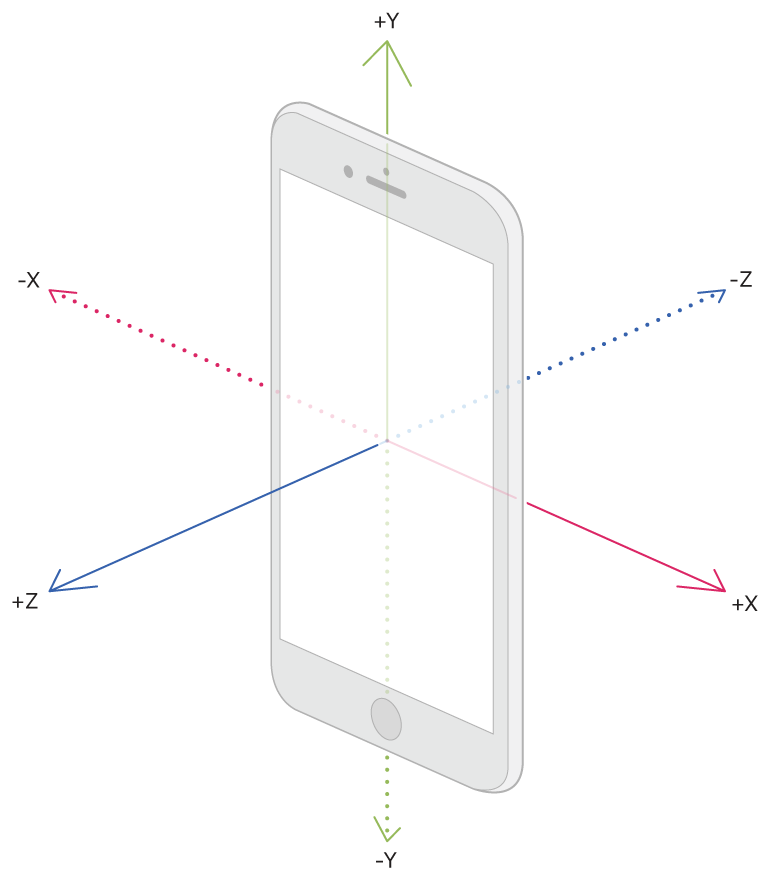
\includegraphics[width=5cm]{images/accelerometer_axes.png}
        \captionof{figure}{Disposizione degli assi dell'accelerometro sullo smartphone.}
        \label{fig:accelerometer_axes}
    \end{minipage}
    \begin{minipage}{.4\textwidth}
        \centering
        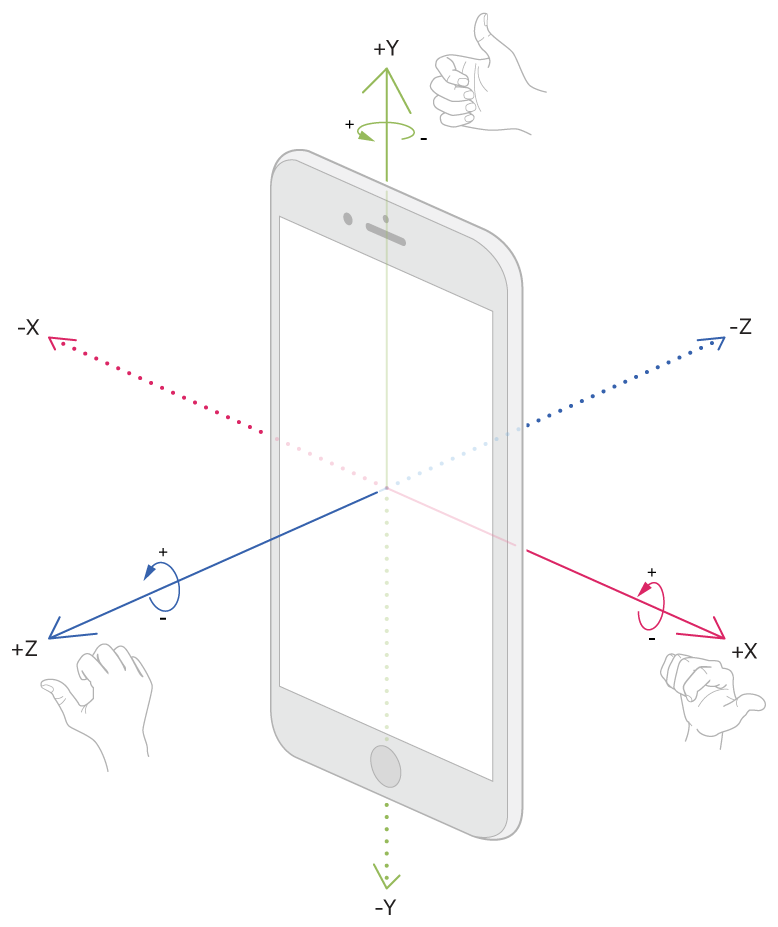
\includegraphics[width=5cm]{images/gyroscope_axes.png}
        \captionof{figure}{Disposizione degli assi del giroscopio sullo smartphone.}
        \label{fig:gyroscope_axes}
    \end{minipage}
\end{figure}

\subsection{Implementazione su iOS}

La prima implementazione del raccoglitore è stata fatta per l'ambiente iOS.\\
\'E stato definita una classe \emph{ParkTypeSampleCollector}, da cui poter creare
istanze di raccoglitori. All'interno dell'app, un raccoglitore viene attribuito ad
un'auto \emph{Car}, in quanto ha lo scopo di raccogliere i dati durante i tragitti 
percorsi da quella determinata macchina.\\
Al \emph{ParkTypeSampleCollector} è stata impostata una cadenza costante di 0.1
secondi, in modo da avere un tasso di campionamento abbastanza elevato, in grado
di distinguere piccole variazioni in campioni consecutivi.\\
Per i singoli campioni è stata definita una struttura \emph{Sample}, contenente
una serie di valori:
\begin{itemize}
    \item \emph{heading}: consiste nell'angolo tra la punta dello smartphone è il nord geografico,
    rappresentato in gradi.
    \item \emph{acceleration}: contiene i tre componenti dell'accelerazione ottenuti attraverso 
    gli accelerometri e processati direttamente dalla libreria \emph{Core Motion}\footnote{\emph{Core Motion} page on Apple's website: 
    \href{https://developer.apple.com/documentation/coremotion}{\underline{link to the page.}}}
    \cite{using_core_motion}. 
    Questo significa che i tre componenti relativi ai tre assi non contengono più
    l'informazione sulla gravità, questa è stata sottratta automaticamente.
    \item \emph{rotationRate}: similmente, contiene i tre componenti estratti dai giroscopi
    e adeguatamente processati.
    \item \emph{speed}: consiste nell'attuale velocità calcolata dal dispositivo ed ottenuta 
    grazie alla libreria \emph{Core Location}\footnote{\emph{Core Location} page on Apple's website: 
    \href{https://developer.apple.com/documentation/corelocation}{\underline{link to the page.}}}
    \cite{introduction_core_location}.
\end{itemize}

Il \emph{ParkTypeSampleCollector} è dotato di un buffer di \emph{Sample} di dimensione fissa.
Questo buffer è utilizzato per salvare la sequenza di campioni che vengono raccolti durante
il tragitto. In quanto l'obiettivo finale è quello di utilizzare i dati per classificare 
il tipo di un parcheggio, è necessario salvare soltanto i campioni che sono stati raccolti 
in momenti temporalmente vicini al termine del parcheggio. Chiaramente non si può sapere a 
priori quanto tempo impiegherà l'utente a parcheggiare, così la raccolta viene avviata
alla partenza dell'auto. Nonostante questo, per evitare di occupare grandi quantità di
memoria con dati che alla fine verranno eliminati, si è pensato di aggiungere campioni al
buffer, fino al suo riempimento, e successivamente aggiungere un potenziale nuovo campione 
rimpiazzando il meno recente presente nel buffer. Questa operazione è stata implementata
in tempo costante, grazie ad un indice utilizzato in aggiunta. Dal momento che non vengono
salvati i timestamp "reali" relativi ai singoli campioni, dei timestamp verranno calcolati
dinamicamente al termine, utilizzando gli indici del buffer e l'intervallo di campionamento.
La dimensione che è stata scelta per il buffer è di 2048 elementi, che si traducono in una
registrazione finale che coprirà un intervallo di tempo che dura al massimo qualche minuto.\\
Il raccoglitore viene azionato ogni volta che passa la quantità di tempo relativo all'
intervallo di campionamento. Ovvero, all'avvio di esso, ha inizio un ciclo che
termina solamente quando l'auto è stata parcheggiata. Ad ogni iterazione viene aggiunto un
nuovo campione al buffer e poi viene effettuata un'attesa, prima che si passi all'iterazione
successiva. L'intero ciclo viene eseguito asincronamente utilizzando la chiamata
\emph{DispatchQueue.global().async} \cite{gcd_basics}, fornita da iOS. Ciò che fa questa funzione è
accodare una funzione, fornita dallo sviluppatore, alla coda di esecuzione globale del
sistema operativo, in maniera asincrona.\\
L'avvio e la terminazione del raccoglitore vengono eseguiti rispettivamente nei metodi 
\emph{unpark()} e \emph{park()} dell'istanza di \emph{Car}. Quindi, quando l'auto 
esce dal parcheggio all'inizio del tragitto e quando parcheggia al termine di esso.

\section{Caricamento dati nel database}

Al termine di ogni registrazione, i dati raccolti devono essere caricati nel database.
Come formato di salvataggio delle registrazioni è stato scelto JSON 
\cite{javascript_object_notation} \cite{json_data_exchanging}. 
Quindi, non appena
il raccoglitore termina la raccolta, il buffer ottenuto deve essere convertito in un 
oggetto JSON (Figura~\ref{fig:esempio_campioni}). In particolare, questo avviene ponendo,
come chiavi dell'oggetto, i timestamp
calcolati rispetto al primo elemento. Ad ogni chiave viene associato un'array di valori, che
contiene tutti i dati ottenuti dal campione di quello specifico istante. Così l'array è
composto da:
\begin{itemize}
    \item \emph{heading}
    \item I tre componenti singoli ottenuti da \emph{acceleration}
    \item I tre componenti singoli ottenuti da \emph{rotationRate}
    \item \emph{speed}
\end{itemize}
Siccome GeneroCity già effettuava una chiamata all'API del backend per registrare dei dati
relativi al parcheggio che è stato appena effettuato, è stato deciso di sfruttare quest'ultima
anche per caricare l'oggetto JSON che contiene i campioni. Così è stato creato un nuovo campo
nel database, relativo al parcheggio e chiamato \emph{parksamples}. All'interno di questo campo
viene salvata la stringa serializzata, ottenuta dall'oggetto JSON.

\begin{figure}
    \centering
    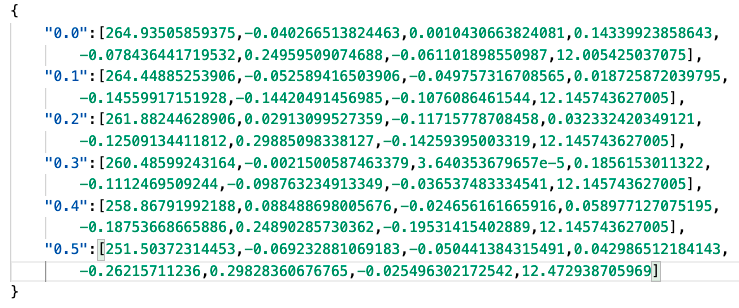
\includegraphics[width=13cm]{images/esempio_campioni.png}
    \caption{Esempio di una registrazione di campioni, sottoforma di oggetto JSON. Ad ogni 
    timestamp, è associato l'array di valori formato rispettivamente da: \emph{heading}, asse X 
    accelerometro, asse Y accelerometro, asse Z accelerometro, asse X giroscopio, asse Y
    giroscopio, asse Z giroscopio, \emph{speed}.}
    \label{fig:esempio_campioni}
\end{figure}

\section{Preparazione dei dati} 

Dal momento che i dati sono stati raccolti quotidianamente, il dataset delle registrazioni
si è andato a popolare di giorno in giorno. In questo modo, è stato possibile effettuare il 
training del modello classificatore di tanto in tanto, al fine di migliorarne le performance
\cite{impact_training_dataset_size}
sempre di più, avendo a disposizione più registrazioni. Per automatizzare il processo di 
preparazione dei dati, è stato creato uno script, composto da moduli, in Python\footnote{
Python's website: 
\href{https://www.python.org}{\underline{link to the page.}}}. Come
precedentemente anticipato, la funzione principale dello script è stata quella di scaricare,
pulire e processare i dati ottenuti. Infatti, ad ogni invocazione esso
\begin{enumerate}
    \item richiede al database e scarica tutte le registrazioni che ancora non sono state 
    salvate in locale;
    \item effettua tutte le procedure di pulitura e processamento dei dati;
    \item prepara i dati per essere utilizzati come input del classificatore e crea una 
    struttura di file CSV \cite{common_format_csv}, con directory classificate in 
    base all'etichetta scelta dall'utente per la registrazione;
\end{enumerate}
Inoltre, insieme allo script è presente un modulo che ha lo scopo di effettuare il plotting
dei dati. Questo plotter è utilizzato per analizzare i dati in maniera visiva ed è in
grado di mostrare i valori uscenti dai vari sensori in diverse modalità e quindi
evidenziando diversi aspetti di essi. Ad esempio, è possibile tracciare valori provenienti
da un componente dell'accelerazione nel tempo, sotto forma di una curva 2D, ma anche i 
punti (formati da tutti i tre componenti) dell'accelerazione stessa, rappresentati in uno 
spazio 3D.

\section{Modelli ML utilizzati} 

Avendo i dati pronti e nel giusto formato, il passo successivo è quello di effettuare il 
training di un modello classificatore.\\
Per creare i modelli è stato deciso di utilizzare la libreria \emph{Create ML}\footnote{
\emph{Create ML} page on Apple's website: 
\href{https://developer.apple.com/documentation/createml}{\underline{link to the page.}}}
\cite{custom_core_ml_models_create_ml} di Apple.
Questa libreria da modo di realizzare nuovi modelli di machine learning con una prospettiva
ad alto livello, permettendo l'utilizzo anche ad utenti che non sono dotati di una conoscenza
molto approfondita a riguardo. Essa offre anche un'interfaccia grafica che rende la creazione 
ancora più intuitiva.\\
Al fine di ottenere un classificatore per tipi di parcheggio, sono stati utilizzati due 
approcci diversi, a partire da due template differenti di \emph{Create ML}:
\begin{itemize}
    \item una rete neurale convoluzionale, utilizzando il \emph{Motion Activity Classifier};
    \item un tree ensemble, utilizzando il \emph{Tabular Classifier}
\end{itemize}
Il motivo per cui sono stati creati due modelli differenti è che il dataset che è stato 
possibile ottenere con un numero molto limitato di utenti disponibili per la raccolta di 
dati, non è composto da un numero di registrazioni sufficentemente grande. Per
questa motivazione, alcuni tipi di modelli hanno ottenuto scarsi risultati nella 
classificazione e si è preferito tentare in diversi modi.

% TODO: maybe add Simulation ...
% TODO: add heading saving ...
